\documentclass[10pt]{article}
\usepackage[a4paper, total={6.5in, 9in}]{geometry}
\usepackage[utf8]{inputenc}
\usepackage{fancyhdr, float}
\usepackage{amsmath, amsthm, amsfonts, amssymb}
\usepackage{xcolor, graphicx}
\usepackage{subfig}

\lhead{Braden Hoagland}
\chead{MATH 490 - HW 6}
\rhead{\today}

\pagestyle{fancy}
\setlength{\parskip}{0.5em}

\renewcommand{\labelenumii}{(\roman{enumii})}
\newcommand{\rr}{\mathscr{R}_0}

\begin{document}
\begin{enumerate}
\item 
\begin{enumerate}
	\item Let $\mu = \mathbb{E}[Y] = 0\cdot 0.4 + 2\cdot 0.6 = 1.2$, then $\mathbb{E}[Z_n]= \mu^n Z_0 = 1.2^n$. Then $\mathbb{E}[Z_n] \geq 10000 \implies n \geq \log_{1.2}(10000) \approx 50.5$, so we expect the number of infected individuals to reach 10000 after about 51 generations.
	\item The probability of extinction is the smallest non-negative solution of $G_Y(\gamma)=\gamma$. Since
		\[
			G_Y(s) = \sum_{k=0}^{\infty} s^k p_k = s^0 p_0 + s^2 p_2 = 0.4 + 0.6s^2,
		\]
		we have
		\[
			\gamma=G_Y(\gamma) \implies \gamma=0.4+0.6\gamma^2 \implies \gamma=\frac{1\pm 0.2}{1.2} = 1, 2/3.
		\]
		Thus the probability of extinction is $2/3$.

	\item A histogram of the simulation is shown below.
		\begin{figure}[H]
			\centering
			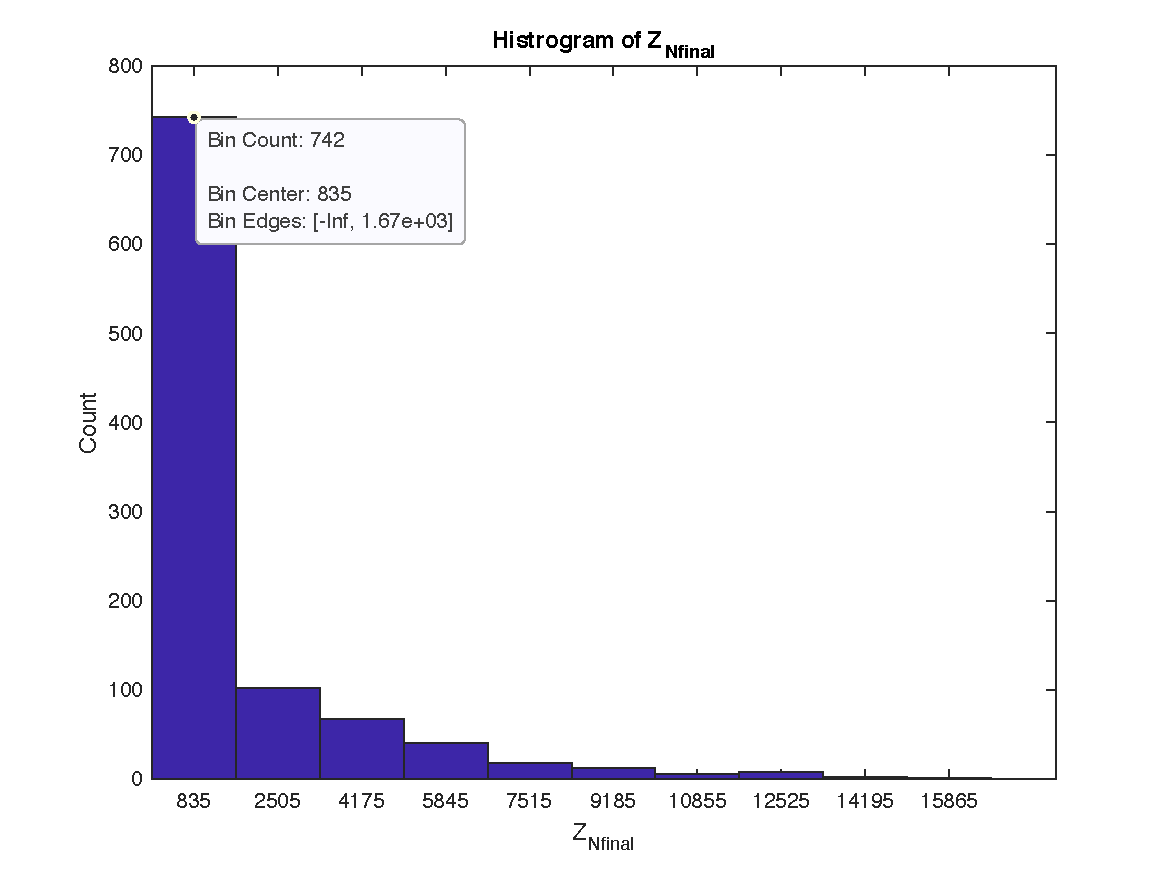
\includegraphics[scale=0.5]{fig/fig1.pdf}
			\caption{1000 samples with final time  $n=40$.}
		\end{figure}

		This shows 742 simulated trajectories going extinct, or 74.2\% of the simulations. The empirical mean of the 1000 samples of $Z_{40}$ is approximately $1295$. Since $\mu = 1.2$, the actual mean is $\mathbb{E}[Z_{40}]=\mu^{40} \approx 1469.$
		
\end{enumerate}

%%%%%%%%%%
% 2
%%%%%%%%%%
\item 
\begin{enumerate}
	\item The offspring distribution should be a weighted average of the moderate and super spreader distributions.
		\[
			\left\{ p_k \right\}_{k=0}^\infty = \left\{ p_0 = 0.88\alpha+0.4(1-\alpha), p_2=0.6(1-\alpha), p_{10}=0.12\alpha \right\}.
		\] 
	
	\item 
		Below are simulated cumulative infectious cases for $\alpha=0$ and $\alpha=1/2$. Note the different scales of each graph. From this we can see
		\begin{enumerate}
			\item When $\alpha=1/2$, the largest outbreaks are significantly larger than than the largest outbreaks when $\alpha=0$, and
			\item Fewer of these large outbreaks occur. A larger percentage of outbreaks die out early on when $\alpha=1/2$.
		\end{enumerate}
		\begin{figure}[H]
			\centering
			\subfloat{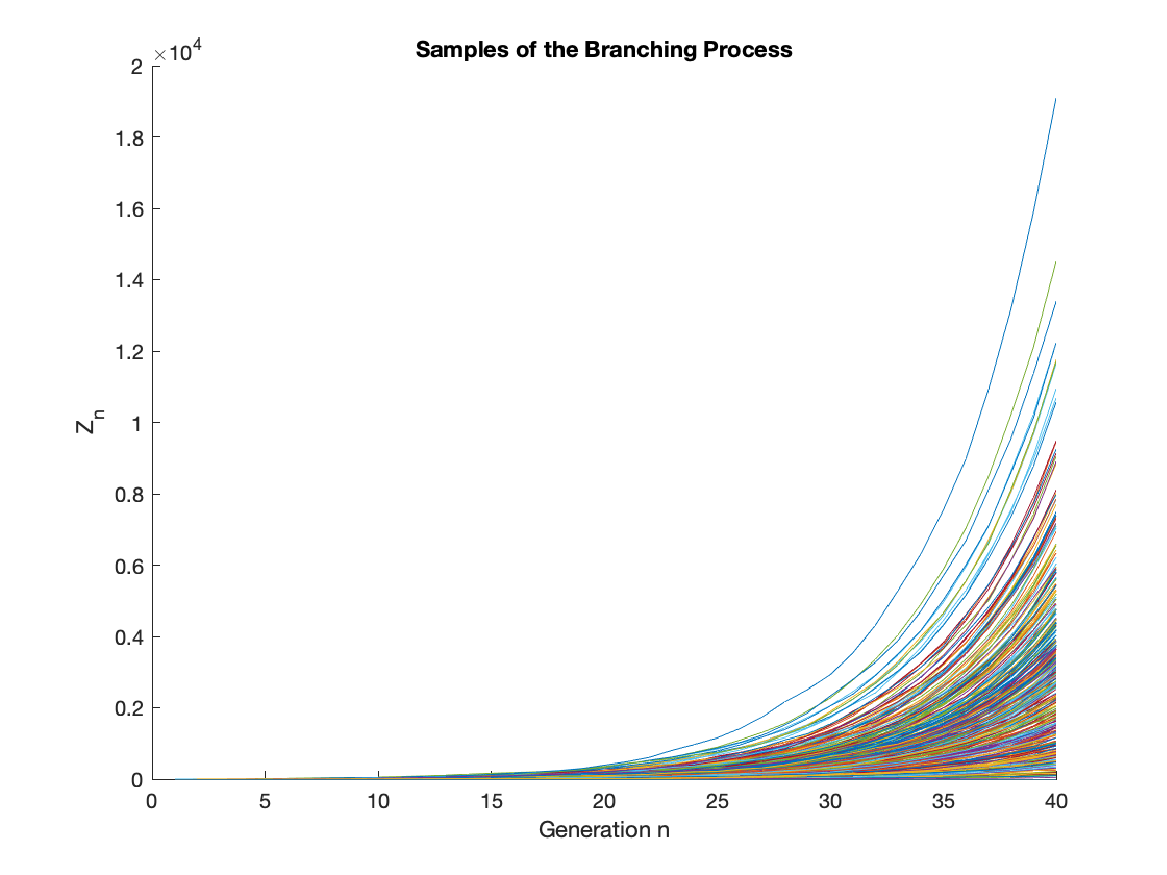
\includegraphics[scale=0.4]{fig/0.pdf}}
			\subfloat{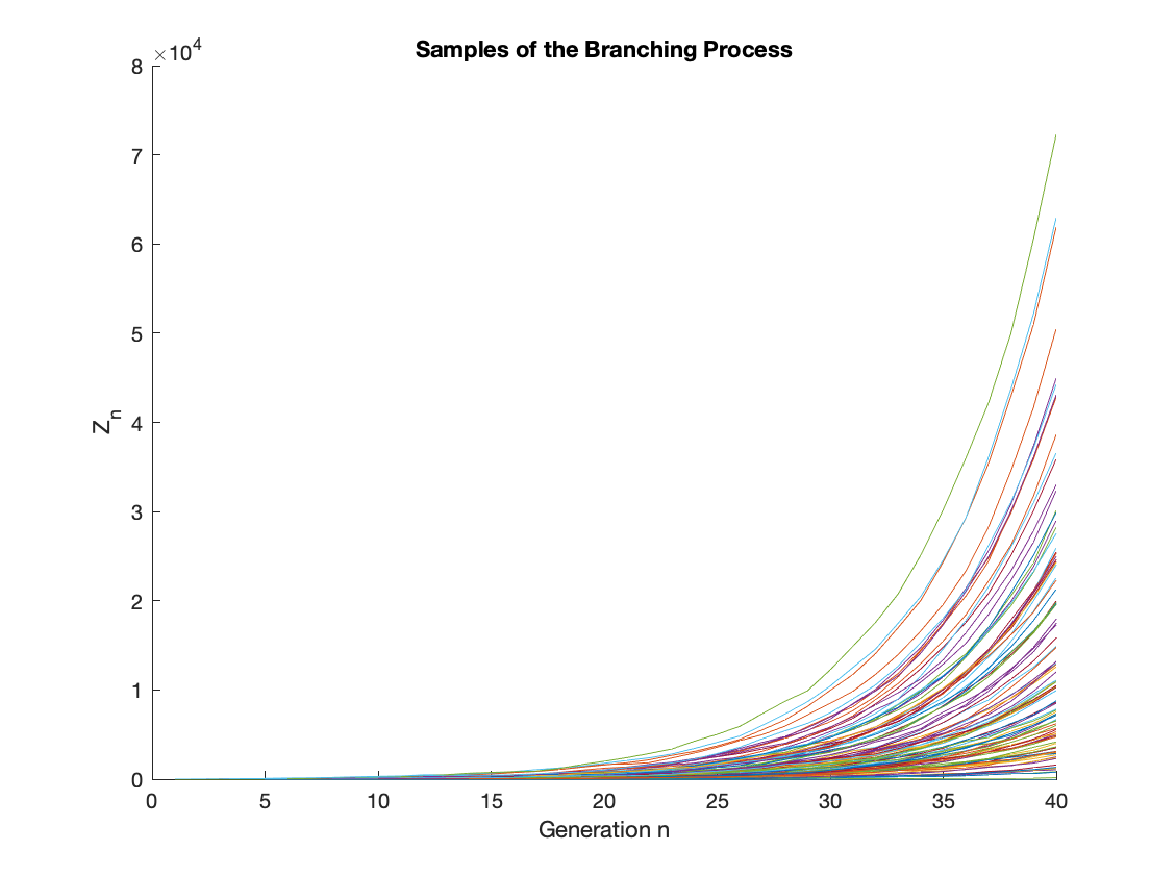
\includegraphics[scale=0.4]{fig/12.pdf}}
			\caption{Left: $\alpha=0$, Right: $\alpha=1/2$.}
		\end{figure}
		Since the growth of these outbreaks is exponential when viewed at a large scale, we can infer that when $\alpha=1/2$, the behavior at early generations is comparable to a highly variant choice of initial condition. With low probability, the disease is initially spread to many people and a large outbreak occurs because the probability of many branches all dying out is small (akin to starting an exponential growth model with a higher initial condition). With high probability, few people contract the disease and it dies out quickly.
		
\end{enumerate}

%%%%%%%%%%
% 3
%%%%%%%%%%
\item
\begin{enumerate}
	\item The generating function for $Y$ is
		\[
			G_Y(s) = \sum_{k=0}^{\infty} s^k p_k = s^0 p_0 + s^2 p_2 = 0.53 + 0.47s^2
		,\]
		so we have
		\[
			\gamma = G_Y(\gamma) \implies \gamma = 0.53 + 0.47 \gamma^2 \implies \gamma = 1 \text{ or } \gamma \approx 1.1.
		\] 
		The minimum of these two roots is $1$, so the extinction probability is 1.

	\item In this example, the outbreak begins with a single infection. This one person is assumed to infect $Y$ people. Since branching process assume that branches grow independently of one another, each of these individuals can then be treated as the original infectious individual of a ``new" outbreak.

		Suppose the original infected person infects people $1$ through $Y$. Let $D_i$ denote the number of people that newly-infected person $ i$ infects, then the total number of infected $D$ can be written recursively as
		\[
		D = 1 + D_1 + D_2 + \cdots + D_Y.
		\] 
		In words, this says that the total number of infected people is equal to the 1 original person infected person plus the number of infected individuals in each of the original $Y$ branches.
	
	\item We can partition this expectation over all possible values of $ Y$.
		\begin{align*}
			\mathbb{E}[D] &= \sum_{y=0}^{\infty} \mathbb{E}[D\;|\;Y=y] \mathcal{P}(Y=y) \\
				      &= \mathbb{E}[D\;|\;Y=0] p_0+\mathbb{E}[D\;|\;Y=2]p_2 \\
				      &= p_0+p_2 \cdot \mathbb{E}[1+D_1+D_2].
				      \intertext{Then since each $D_i$ has the same distribution as $D$, and by linearity of expectation, this becomes}
			\mathbb{E}[D] &= p_0 + p_2 + 2p_2 \cdot \mathbb{E}[D] \\
			\mathbb{E}[D] &= \frac{p_0+p_2}{1-2p_2} \\
			\mathbb{E}[D] &= \frac{0.53 + 0.47}{1-0.94} = \frac{1}{0.06} \approx 16.7.
		\end{align*}
		Thus we expect between 16 and 17 people to become infected during this outbreak.
\end{enumerate}


\end{enumerate}
\end{document}
